\documentclass[12pt]{article}
\usepackage[letterpaper]{geometry}                                              
                                                                                
%%% This file can never be completed.
%%% If you need something but cannot find it,
%%% contact the TA Favonia!

%%%%%%%%%%%%%%%%%%%%%%%%%%%%%%%%%%%%%%%%
% Basic packages
%%%%%%%%%%%%%%%%%%%%%%%%%%%%%%%%%%%%%%%%
\usepackage{amsmath,amsthm,amssymb}
\usepackage{mathtools}
\usepackage{etoolbox}
\usepackage{fancyhdr}
\usepackage{mathpartir}
%\usepackage[usenames,dvipsnames]{xcolor}
\usepackage[colorlinks=true,urlcolor=blue,linkcolor=blue,citecolor=blue]{hyperref}
\usepackage{xspace}
\usepackage{comment}
\usepackage{url} % for url in bib entries


%%%%%%%%%%%%%%%%%%%%%%%%%%%%%%%%%%%%%%%%
% Acronyms
%%%%%%%%%%%%%%%%%%%%%%%%%%%%%%%%%%%%%%%%
\usepackage[acronym, shortcuts]{glossaries}

\newacronym{HoTT}{HoTT}{homotopy type theory}
\newacronym{IPL}{IPL}{intuitionistic propositional logic}
\newacronym{TT}{TT}{intuitionistic type theory}
\newacronym{LEM}{LEM}{law of the excluded middle}
\newacronym{ITT}{ITT}{intensional type theory}
\newacronym{ETT}{ETT}{extensional type theory}
\newacronym{NNO}{NNO}{natural numbers object}

% Make \ac robust.
\robustify{\ac}

%%%%%%%%%%%%%%%%%%%%%%%%%%%%%%%%%%%%%%%%
% Fancy page style
%%%%%%%%%%%%%%%%%%%%%%%%%%%%%%%%%%%%%%%%
\pagestyle{fancy}
\newcommand{\metadata}[2]{
  \lhead{}
  \chead{}
  \rhead{\bfseries Homotopy Type Theory}
  \lfoot{#1}
  \cfoot{#2}
  \rfoot{\thepage}
}
\renewcommand{\headrulewidth}{0.4pt}
\renewcommand{\footrulewidth}{0.4pt}


\newrobustcmd*{\vocab}[1]{\emph{#1}}
\newrobustcmd*{\latin}[1]{\textit{#1}}

%%%%%%%%%%%%%%%%%%%%%%%%%%%%%%%%%%%%%%%%
% Customize list enviroonments
%%%%%%%%%%%%%%%%%%%%%%%%%%%%%%%%%%%%%%%%
% package to customize three basic list environments: enumerate, itemize and description.
\usepackage{enumitem}
\setitemize{noitemsep, topsep=0pt, leftmargin=*}
\setenumerate{noitemsep, topsep=0pt, leftmargin=*}
\setdescription{noitemsep, topsep=0pt, leftmargin=*}

%%%%%%%%%%%%%%%%%%%%%%%%%%%%%%%%%%%%%%%%
% Some really basic macros.
% (Lots of them were stolen from HoTT/Book.)
% See macros.tex in HoTT/book.
%
% This is a mess.  Needs clean-ups.
%%%%%%%%%%%%%%%%%%%%%%%%%%%%%%%%%%%%%%%%
\newrobustcmd*{\ctx}{\Gamma}
\newrobustcmd*{\entails}{\vdash}

\newrobustcmd*{\judgmentfont}[1]{{\normalfont\sffamily #1}}
\newrobustcmd*{\postfixjudgment}[1]{%
  \relax\ifnum\lastnodetype>0\mskip\medmuskip\fi
  \text{\judgmentfont{#1}}%
}
\newrobustcmd*{\prop}{\postfixjudgment{prop}}
\newrobustcmd*{\true}{\postfixjudgment{true}}
\newrobustcmd*{\type}{\postfixjudgment{type}}
\newrobustcmd*{\context}{\postfixjudgment{ctx}}

\newrobustcmd*{\truth}{\top}
\newrobustcmd*{\conj}{\wedge}
\newrobustcmd*{\disj}{\vee}
\newrobustcmd*{\falsehood}{\bot}
\newrobustcmd*{\imp}{\supset}
\newrobustcmd*{\zero}{0}

%%% Judgmental equality
\newrobustcmd*{\jdeq}{\equiv}
%%% Definition
\newrobustcmd*{\defeq}{\vcentcolon\equiv}
%%% Binary sums
\newrobustcmd*{\inlsym}{{\mathsf{inl}}}
\newrobustcmd*{\inrsym}{{\mathsf{inr}}}
\newrobustcmd*{\inl}{\ensuremath\inlsym\xspace}
\newrobustcmd*{\inr}{\ensuremath\inrsym\xspace}
%%% Booleans
\newrobustcmd*{\ttsym}{{\mathsf{tt}}}
\newrobustcmd*{\ffsym}{{\mathsf{ff}}}
%%% Pairs
\newrobustcmd*{\pair}{\ensuremath{\mathsf{pair}}\xspace}
\newrobustcmd*{\tuple}[2]{(#1,#2)}
\newrobustcmd*{\proj}[1]{\ensuremath{\mathsf{pr}_{#1}}\xspace}
%% Empty type
\newrobustcmd*{\abort}[1]{\ensuremath{\mathsf{abort}_{#1}}}
%%% Path concatenation
\newrobustcmd*{\concat}{%
  \mathchoice{\mathbin{\raisebox{0.5ex}{$\displaystyle\centerdot$}}}%
  {\mathbin{\raisebox{0.5ex}{$\centerdot$}}}%
  {\mathbin{\raisebox{0.25ex}{$\scriptstyle\,\centerdot\,$}}}%
  {\mathbin{\raisebox{0.1ex}{$\scriptscriptstyle\,\centerdot\,$}}}
}
%%% Transport (covariant)
\newrobustcmd*{\trans}[2]{\ensuremath{{#1}_{*}\mathopen{}\left({#2}\right)\mathclose{}}\xspace}
% Natural numbers objects
\newrobustcmd*{\Nat}{\mathsf{Nat}}
\newrobustcmd*{\rec}{\ensuremath{\mathsf{rec}}\xspace}
% Sequence
\newrobustcmd*{\Seq}{\ensuremath{\mathsf{Seq}}\xspace}
% Identity type
\newrobustcmd*{\Id}[1]{\ensuremath{\mathsf{Id}_{#1}}\xspace}
% Reflection
\newrobustcmd*{\refl}[1]{\ensuremath{\mathsf{refl}_{#1}}\xspace}
\newrobustcmd*{\J}{\ensuremath{\mathsf{J}}\xspace}

% fst,snd,case,id
\newrobustcmd*{\fst}{\textsf{fst}}
\newrobustcmd*{\snd}{\textsf{snd}}
\DeclareMathOperator{\case}{\textsf{case}}
\DeclareMathOperator{\caseif}{\textsf{if}}
\DeclareMathOperator{\casesplit}{\textsf{split}}
\DeclareMathOperator{\ttrue}{\textsf{tt}\xspace}
\DeclareMathOperator{\ffalse}{\textsf{ff}\xspace}
\newrobustcmd*{\id}{\textsf{id}}

\newrobustcmd*{\op}[1]{\operatorname{#1}}

\newrobustcmd*{\universe}{\mathcal{U}}

%inductive types
\newrobustcmd*{\ind}{\ensuremath{\mathsf{ind}}\xspace}
%higher inductive types
%interval
\newrobustcmd*{\interval}{\ensuremath{I}\xspace}
\newrobustcmd*{\seg}{\ensuremath{\mathsf{seg}}\xspace}
%circle
\newrobustcmd*{\Sn}{\mathbb{S}}
\newrobustcmd*{\base}{\ensuremath{\mathsf{base}}\xspace}
\newrobustcmd*{\lloop}{\ensuremath{\mathsf{loop}}\xspace}
                                                                  
                                                                                
\usepackage{proof-dashed}                                                       
\usepackage{tikz-cd}                                                            
\usepackage{amsmath}                                                            
\usepackage{lmodern}                                                            
\usepackage{microtype}                                                          

\metadata{Lewis and Tassarotti}{2013/10/21 and 2013/10/23}

\newtheorem{thm}{Theorem}
\newtheorem{eg}{Example}
\newcommand{\ap}{\mathsf{ap}}
\newcommand{\apd}{\mathsf{apd}}
\newcommand{\tr}{\mathsf{tr}}
\newcommand{\iseq}{\mathsf{isequiv}}
\newcommand{\qinv}{\mathsf{qinv}}
\newcommand{\happ}{\mathsf{happly}}
\newcommand*{\comp}{\mathbin{\circ}}

\newtheorem*{remark}{Remark}
\newtheorem*{proposition}{Proposition}
\newtheorem*{exercise}{Exercise}
\newtheorem*{lemma}{Lemma}

\begin{document}
\title{15-819 Homotopy Type Theory Lecture Notes} 
\author{Robert Lewis and Joseph Tassarotti}
\date{October 21 and 23, 2013}

\maketitle

\section{Paths-over-Paths}\label{}

Recall that last time we explored the higher groupoid structure of types, and
showed that for non-dependent maps, $\ap$ preserves this structure.  Now, in
the case where we have a dependent function $f : \Pi x: A.B$, we would like to
similarly state that $f$ maps equals to equals, so that given a path $p :
\Id{A}(M,N)$, there is some map which takes in $p$ and gives a path between $f
M$ and $f N$. However, because $f$ is dependent, $f M : [M/x]B$ and $f N :
[N/x] B$.  Although these types are related, they are not equal, so we cannot
talk about propositional equality between $f M$ and $f N$.

In earlier lectures, we defined $\tr[x.B]p : [M/x] B \to [N/x] B$, often
written as $p_*$, which lifts the path $p$ to a mapping between the fibers
$[M/x] B$ and $[N/x] B$. Since $p_*(f M)$ and $f N$ share the same type, we can
meaningfully talk about equality between them. We can now define a map $\apd_f
: \Pi p: \Id{A}(M, N). \Id{[N/x]B}(p_* (f M), f N)$ by
%
\[ \apd_f p := \J[m.n.z. \Id{[n/x]B}(z_{*}(f m), f n)](p ; m. \refl{[m/x]B}(m)) \]
%

This has the appropriate type because when the path is simply $\refl{A}(M)$, we
have that $(\refl{A}(M))_* \jdeq \refl{[M/x]B}(f M)$. See
figure~\ref{fig:paths-over-paths} for a pictorial representation of this. 

Now, since $p_*^{-1}$ gives a map between the fibers going the other way, we
could just as well have defined an analogous term $\apd_f' : \Id{A}(M, N) \to
\Id{[M/x]B}(f M, p_*^{-1}(f N))$. Moreover, we have that
%
\[
\begin{array}{lcl}
\ap_{p_*^{-1}} (\apd_f p) &:& \Id{[M/x]B}(p_*^{-1} (p_* (f M)), p_*^{-1} (f N))  \\
                          & &  \ \ \jdeq \Id{[M/x]B}(f M, p_*^{-1} (f N)) \\
\\
\ap_{p_*} (\apd_f p^{-1}) &:& \Id{[N/x]B}(p_* (f M)), p_* (p_*^{-1} (f N))) \\
                          & &  \ \ \jdeq \Id{[N/x]B}(p_* (f M), f N) \\

\end{array}
\]
%
which shows that these two theorems imply one another. 

The lack of symmetry in the types of $\apd_f$ and $\apd_f'$ is somewhat awkward
when developing machine checked proofs. It's more convenient to define a
symmetric notation, $f(M) =_p^{x. B} f(N) \defeq Id{[N/x]B}(p_* (f M), f N)$,
which we read as ``$f(M)$ and $f(N)$ are correlated by $p$" . This corresponds
to the type of paths \emph{over} the path $p$. Using this notation, we 
can prove theorems about this type like:

\[
\begin{array}{lcl}
\text{sym}_{\text{corr}} & : & Q =_p^{x.B} R \ \to \ R =_{p^{-1}}^{x.B} Q \\
\\
\text{trans}_{\text{corr}} & : & Q =_p^{x.B} R \ \to R =_q^{x.B} S \to Q =_{p \concat q}^{x.B} S 
\end{array}
\]
%


\begin{figure}
\label{fig:paths-over-paths}
\begin{center}
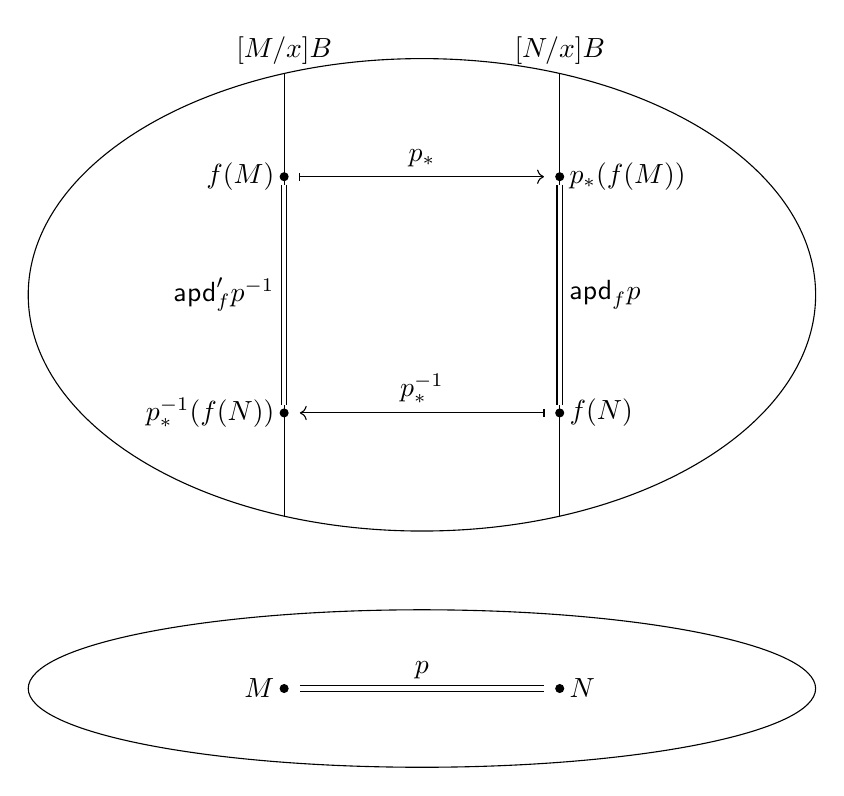
\begin{tikzpicture}
   \draw (0, 0) ellipse (5cm and 3cm);
   \draw (0, -5cm) ellipse (5cm and 1cm);

   \draw [double equal sign distance] (-1.55 cm, -5cm) --  (1.55 cm, -5cm);
   \node [above] at (0 cm, -5cm) {$p$};
   \draw [fill] (-1.75cm, -5cm) circle [radius=.05cm];
   \node [left] at (-1.75cm, -5cm) {$M$};
   \draw [fill] (1.75cm, -5cm) circle [radius=.05cm];
   \node [right] at (1.75cm, -5cm) {$N$};

   \draw (-1.75 cm, -2.8102cm) -- (-1.75cm, 2.8102cm);
   \node [above] at (-1.75 cm, 2.8cm) {$[M/x]B$};
   \draw (1.75 cm, -2.8102cm) -- (1.75cm, 2.8102cm);
   \node [above] at (1.75 cm, 2.8cm) {$[N/x]B$};

   % p_* 
   \draw [fill] (-1.75cm, 1.5 cm) circle [radius=.05cm];
   \node [left] at (-1.75cm, 1.5cm) {$f(M)$};
   \draw [fill] (1.75cm, 1.5 cm) circle [radius=.05cm];
   \node [right] at (1.75cm, 1.5cm) {$p_*(f(M))$};
   \node [above] at (0 cm, 1.5cm) {$p_*$};
   \draw [->] (-1.55 cm, 1.5cm) --  (1.55 cm, 1.5cm);
   \draw (-1.55cm, 1.45cm) -- (-1.55cm, 1.55cm);

   % p_* inverse
   \draw [fill] (-1.75cm, -1.5 cm) circle [radius=.05cm];
   \node [left] at (-1.75cm, -1.5cm) {$p_*^{-1}(f(N))$};
   \draw [fill] (1.75cm, -1.5 cm) circle [radius=.05cm];
   \node [right] at (1.75cm, -1.5cm) {$f(N)$};
   \node [above] at (0 cm, -1.5cm) {$p_*^{-1}$};
   \draw [->]  (1.55 cm, -1.5cm) -- (-1.55 cm, -1.5cm) ;
   \draw (1.55cm, -1.45cm) -- (1.55cm, -1.55cm);


   \draw [double equal sign distance, shorten <= .15 cm, shorten >= .15 cm] (1.75 cm, 1.55cm) --  (1.75 cm, -1.55cm);
   \node [right] at (1.75cm, 0cm) {$\apd_f p$};
   \draw [double equal sign distance, shorten <= .15 cm, shorten >= .15 cm] (-1.75 cm, 1.55cm) --  (-1.75 cm, -1.55cm);
   \node [left] at (-1.75cm, 0cm) {$\apd_f' p^{-1}$};


\end{tikzpicture}
\end{center}
\caption{Paths-over-paths}

\end{figure}


\section{Equivalence of Types}

\subsection{Motivation}

We start by informally recalling some notions of equivalence that are commonly
used in mathematics:

\begin{enumerate}

\item \emph{Biconditional propositions}: Given two propositions $p$ and $q$
such that $p \imp q$ and $q \imp p$, we might wish to say that $p = q$,
because these two propositions are logically equivalent. In classical logic,
this makes sense, because $p$ and $q$ are both either equal to true or equal
false. To quote Whitehead and Russell~\cite[p.115]{Whitehead63}:

\begin{quotation}

When each of two propositions implies the other, we say that the two are
\emph{equivalent}, which we write ``$p \jdeq q$'' \dots It is obvious that two
propositions are equivalent when, and only when, both are true or both are
false\dots

We shall give the name of a \emph{truth-function} to a function
$f(p)$ whose argument is a proposition, and whose truth-value
depends only upon the truth-value of its argument. All the functions
of a proposition with which we shall be specially concerned will be
truth-functions, \emph{i.e.} we shall have
%
\begin{equation*}
p \jdeq q \ . \imp \ . f(p) \jdeq f(q) . 
\end{equation*}
%
\end{quotation}

This means that for Whitehead and Russell, if $p$ and $q$ are logically
equivalent, then they are indiscernible. However, in the proof relevant setting
of type theory, this is not the case, because these types classify particular
pieces of data.  Although terms of the type $f : p \to q$ and $g : q \to p$
give us ways to interconvert proofs of $p$ and $q$, a proof of $p$ is not by
itself a proof of $q$.  Moreover, it need not even be the case that $f$ and $g$
are inverses of each other.

\item \emph{Isomorphic sets}: In set theory, we say that two sets $A$ and $B$
are \emph{isomorphic} if there is a bijection between them. That is, there are
functions $f : A \to B$ and $g : B \to A$ such that $g(f(a)) = a$ and $f(g(b))
= b$. In many contexts, it is not relevant for us to distinguish between
isomorphic sets. However, in ZF set theory, just because two sets are
isomorphic does not mean they are indiscernible, so we cannot regard them
as equal.

This is a larger symptom of the fact that although ZF set theory lets us encode
the structures of mathematics, it does not support abstraction. Propositions
like $0 \in 1$ are perfectly well-formed, and are even true for most encodings
of the natural numbers as sets. As de Bruijn points out~\cite{deBruijn95},
these artifacts of a particular encoding contradict the way we conceptually
think of mathematics\footnote{A portion of this passage is quoted in
\cite{Lamport99}, which contains an interesting discussion about some
advantages and disadvantages of types and sets.}:
%
\begin{quotation}
In our mathematical culture we have learned to keep things apart. If we have a
rational number and a set of points in the Euclidean plane, we cannot even
imagine what it means to form the intersection. The idea that both might have
been coded in ZF with a coding so crazy that the intersection is \emph{not
empty} seems to be ridiculous\dots

A very clear case of thinking in terms of types can be found in Hilbert's
axiomatization of geometry. He started by saying that he assumes there are
certain things which will be called \emph{points} and certain things to be
called \emph{lines}. Nothing is said about the nature of these things.
\end{quotation}
%
Type theory rules out statements like $0 \in 1$ as ill-formed. As we shall see,
this same facility for abstraction allows us to give a more suitable treatment
of equivalence.

\end{enumerate}

Now, we turn to the question of equivalences of types. Applying our na\"ive
intuition of regarding types as sets, we might say that types are isomorphic
precisely when there is a bijection between them. In ITT, this will work for
types corresponding to first order data, but we encounter problems when
considering functions.

More precisely, to show that $A \to B$ is isomorphic to $C \to D$, we need to
construct functions $F: (A \to B) \to (C \to D)$ and $G: (C \to D) \to (A \to
B)$ such that for all $f : A \to B$ and $g : C \to D$, $G(F(f)) = f$ and
$F(G(g)) = g$. In a set-theoretic setting, it would suffice to show that for
all $x \in A$, $G(F(f))(x) = f(x)$, and similarly for $F \circ G$. However, in
ITT we lack function extensionality, this is not enough. We need to show that
$G \circ F$ maps $f$ precisely back to itself.  One might try to resolve this
by quotienting by extensionality or adding in an axiom of extensionality.

However, the problem becomes even more difficult when considering universes.
We would need to show that for each type $A$ in the universe, $G(F(A)) = A$.
Just as with functions, where we were really interested in showing that $G
\circ F$ mapped a function to something that was extensionally equivalent, here
we want $G(F(A))$ to itself be isomorphic to $A$ not equal.

\subsection{Homotopy Equivalence}

We now introduce the notion the notion of a \emph{homotopy}. Given two
functions $f, g : A \to B$, a homotopy from $f$ to $g$ is a term with type $\Pi
x:A.  \Id{B} (f x, g x)$. We introduce the notation $f\sim_{A \to B} g$ for the
type of homotopies from $f$ to $g$. If this type is inhabited, we say that $f$
is ``homotopic to'' $g$.

Now, given $H : f\sim_{A \to B}$, we have that for all $x:A$, $f x =_B g x$.
But in fact there is something more going on: $H$ is \emph{dependently
functorial} in $x:A$. That is, $H$ respects paths between inhabitants in $A$
and $B$.  This property is also called \emph{naturality}; we can say that $H$
is a sort of polymorphism in $x:A$. This means that the following diagram
commutes:

\begin{center}
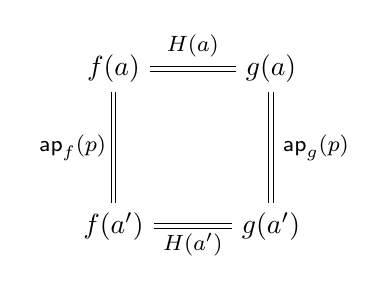
\begin{tikzpicture}[node distance=2cm, auto]
 \node (UL) {$f(a)$};
 \node (UR) [right of=UL] {$g(a)$};
 \node (LL) [below of=UL] {$f(a')$};
 \node (LR) [below of=UR] {$g(a')$};
 
 \draw[transform canvas={yshift=0.2ex},-] (UL) to node {\footnotesize $H(a)$} (UR);
 \draw[transform canvas={xshift=0.2ex},-] (UL) to node [swap] {\footnotesize $\ap_f(p)$} (LL);
 \draw[transform canvas={yshift=0.2ex},-] (LL) to node [swap] {\footnotesize $H(a')$} (LR);
 \draw[transform canvas={xshift=0.2ex},-] (UR) to node {\footnotesize $\ap_g(p)$} (LR);
 
 \draw[transform canvas={yshift=-0.2ex},-] (UL) to node {} (UR);
 \draw[transform canvas={xshift=-0.2ex},-] (UL) to node [swap] {} (LL);
 \draw[transform canvas={yshift=-0.2ex},-] (LL) to node [swap] {} (LR);
 \draw[transform canvas={xshift=-0.2ex},-] (UR) to node {} (LR);
\end{tikzpicture}
\end{center}


\subsection{Basic Properties of Equivalence}\label{subsec:equiv}

For a function $f:A \to B$, we define an \emph{equivalence} between $A$ and
$B$, by $$\iseq(f)\defeq (\Sigma g: B\to A.f\comp g \sim \id_B)\times (\Sigma
h: B\to A.h\comp f \sim \id_A).$$
  
 The proposition expressing that two types $A$ and $B$ are equivalent, written
$A \simeq B$ b, is $$A\simeq B\defeq \Sigma f: A\to B.\iseq(f).$$
  
Since we are in a proof-relevant setting, the information that $A\simeq B$ 
consists of five things:
\begin{itemize}
 \item A function $f:A\to B$
 \item A function $g: B\to A$
 \item A proof $\alpha: \Pi y:B.f(g(y)) =_B y$
 \item A function $h: B\to A$
 \item A proof $\beta: \Pi x:A.h(f(x)) =_A x$
\end{itemize}

To prove that $A\simeq B$, we need to provide all of these as evidence, and from
evidence that $A\simeq B$, we can extract all of these.
  
 We will also be interested in the notion of a \emph{quasi-inverse}:
  $$\qinv(f)\defeq \Sigma g:B\to A.(f\comp g\sim \id_B \times g\comp f\sim \id_A).$$
  
As one might hope, the notions of equivalence and quasi-inverse are very closely related.
One can prove the following properties:

\begin{enumerate}
 \item For every $f:A\to B$, there is a function $\qinv(f) \to \iseq(f)$.
 \item For every $f:A\to B$, there is a function $\iseq(f) \to \qinv(f)$.
\end{enumerate}

This means that the two notions are logically equivalent: a function is an equivalence
if and only if it has a quasi-inverse. In addition, we can show that $\iseq(f)$ 
expresses an HPROP: that is, up to higher homotopy, there is only one proof of this fact.
This will become important later.

\subsection{Function extensionality}

The axiom of function extensionality allows us to show that the $(f =_{A \to B}
g) \simeq (f \sim_{A \to b} g)$.  Even without the axiom, we can define
the map $$ \happ: f =_{A\to B} g \to f\sim_{A\to B} g$$

Now, the axiom says that the above map is an equivalence: if we have a proof of
$f \sim_{A\to B} g$, we may assume that we have a proof of $f =_{A\to B} g$.
This is not necessarily provable without the axiom. For example, in the natural
number type, $\lambda x.0+x \sim_{N\to N} \lambda x.x$, but since addition was
defined inductively on the second argument, we cannot find a path between them.

\subsection{Exercises}
The following propositions are left as exercises, with the first one begun for explanatory
purposes:

\begin{enumerate}
 \item Show that $\id_A: A\to A$ is an equivalence.
 
 To do this, we need four pieces of information:
 \begin{enumerate}
  \item $g: A\to A$. Take this to be $\id_A$.
  \item A proof $\alpha: \Pi y:A. \id_A(g (y)) =_A y$.
  \item $h: A\to A$. Again, take this to be $\id_A$.
  \item A proof $\beta: \Pi x:A. h(\id_A(x)) =_A x$.
 \end{enumerate}

 \item If $f: A\to B$ is an equivalence, then there is $f^{-1}: B\to A$ (given by 
 the quasi-inverse of $f$) that is also an equivalence.
 
 \item If $f: A\to B$ and $g: B\to C$ are equivalences, then so is $g\comp f: A\to C$.
\end{enumerate}



\section{Structure of Paths in Types}

We want to examine the paths inside certain types. For the negative types, this will be
relatively simple. For the positive types, it will be much harder. There are many outstanding
open problems within the positive types.

\subsection{Product Types}
We start by examining the paths in $\Id{A\times B}(\_,\_)$. 

There is a function $f$ such that
$$f: \Id{A\times B}(x,y) \to (\Id{A}(\pi_1 x, \pi_1 y) \times \Id{B}(\pi_2 x,\pi_2 y)).$$

Specifically,

$$f\defeq \lambda p.\langle \ap_{\pi_1} (p) , \ap_{\pi_2} (p) \rangle$$

Roughly speaking, if $x =_{A\times B} y$, then $\pi_1 x =_A \pi_1 y$ and $\pi_2 x =_B \pi_2 y$.

\begin{proposition} $f$ is an equivalence:
 $\Id{A\times B}(x,y) \simeq \Id{A}(\pi_1 x, \pi_1 y) \times \Id{B}(\pi_2 x, \pi_2 y)$.
\end{proposition}

\begin{proof}
 As noted in Section 2, it suffices to produce a quasi-inverse for $f$.
 We need to construct three objects:
 \begin{enumerate}
  \item $g: ( \Id{A}(\pi_1 x, \pi_1 y) \times \Id{B}(\pi_2 x, \pi_2 y) ) \to \Id{A\times B} (x,y)$
  \item $\alpha: g(f(p)) =_{\Id{A\times B} (x,y)} p$
  \item $\beta: f(g(q)) =_{\Id{A}(\pi_1 x,\pi_1 y)\times \Id{B}(\pi_2 x,\pi_2 y)} q$
 \end{enumerate}
 We construct these as follows:
 \begin{enumerate}
  \item We define two auxiliary functions
  $$\pair \defeq \lambda x \lambda y \langle x, y \rangle : A\to B\to A\times B$$
  and
  $$\ap2_f: \Id{}(x,x') \to \Id{}(y,y') \to \Id{}(f x y, f x' y')$$ 
  %Should we fill this out more? Bob left it as an exercise.
  
  Using these, we can then define
  $$g\defeq \lambda \langle p,q \rangle .\ap2_\pair p q$$.
  
  \item To define $\alpha$, it suffices (by FUNEXT) to show:
  \begin{itemize}
   \item $\eta: \Pi p(\ap2_\pair (\ap_{\pi_1}(p), \ap_{\pi_2}(p)) = p)$
   \item $\beta_1: \Pi p \Pi q (\ap_{\pi_1} (\ap2_\pair p q) = p)$
   \item $\beta_2: \Pi p \Pi q (\ap_{\pi_2} (\ap2_\pair p q) = q)$
  \end{itemize}

  By path induction, we need to find $R$ such that
  $$x:A\times B \entails R:(\ap2_\pair(\ap_{\pi_1}(\refl{}(x)),\ap_{\pi_2}(\refl{}(x))))=\refl{}(x)$$
  
  Then,
  $$\eta\defeq J[\ ](p; x.R).$$
  
  By our earlier definition of $\ap$\footnote{
  This is a striking example of anti-modularity. One has no reason to expect that this 
  equality should hold definitionally; it depends essentially on how $\ap$ was defined, 
  not just on its type. It would be nice to avoid this kind of code-on-code dependency,
  since ``the proof should not have to know about the computation."
  }, we have that
  \begin{align*}
   \ap_{\pi_1}(\refl{}(x))\equiv &\ \refl{}(\pi_1(x)) \\
   \ap_{\pi_2}(\refl{}(x))\equiv &\ \refl{}(\pi_2(x))\text{, and from these,} \\
   \ap2_\pair(\refl{}(\pi_1(x))) (\refl{}(\pi_2(x))) \equiv &\ \refl{}\langle \pi_1(x),\pi_2(x)\rangle \\
   \equiv &\ \refl{}(x)
  \end{align*}

  
  \item The constructions of $\beta_1$ and $\beta_2$ are similar and left as exercises.
 \end{enumerate}


\end{proof}

\subsection{Coproduct Types}
Similarly, we can look into $\Id{A+B}(x,y)$. Intuitively speaking, we would like to say that
any path in the space $A+B$ is either a path in $A$ or a path in $B$; we would never expect to have
a path (equation) between an $\inl(a)$ and an $\inl(b)$.

We would like to prove the following facts:

\begin{align*}
 \Id{A+B}(\inl(a),\inl(a'))\simeq &\ \Id{A}(a,a') \\
 \Id{A+B}(\inr(b),\inr(b'))\simeq &\ \Id{B}(b,b') \\
 \Id{A+B}(\inl(a),\inr(b))\simeq &\ 0 \\
 \Id{A+B}(\inr(a),\inl(b))\simeq &\ 0
\end{align*}

Proving this requires a bit of a trick.

Suppose we wanted to prove the first equivalence alone.
The right-to-left direction is simple. For the left-to-right direction, we need to exhibit
$$p: \Id{A+B}(\inl(a),inl(a'))\entails R:\Id{A}(a,a').$$

$R$ must be a path induction on $p$, of the form $R=J[C](p,\_)$ for some motive $C$.
The conclusion of this path induction will be of the form $C(\inl(a),\inl(a'),p)$.
But what we need is $\Id{A}(a,a')$ (note the lack of $\inl$). One might try to define
something like $D(u,v)=\Id{A}(\mathsf{outl}(u),\mathsf{outl}(v))$, but this cannot exist,
since $\mathsf{outl}$ cannot be a total function.

This approach, then, will not work. Instead, we must take a different approach. We will
find a motive $F: (A+B)\times (A+B) \to \mathcal{U}$ such that:
\begin{align*}
 F(\inl(a),\inl(a'))\equiv &\ \Id{A}(a,a') \\
 F(\inr(b),\inr(b'))\equiv &\ \Id{B}(b,b') \\
 F(\inl(a),\inr(b)) \equiv &\ 0 \\
 F(\inr(a),\inl(b)) \equiv &\ 0
\end{align*}

Such an $F$ expresses all of the desired properties of the coproduct.

\begin{exercise}Define such an $F$ by ``double induction.''
 
\end{exercise}

The following lemma expresses the subgoal of our path induction with motive $F$:
\begin{lemma}
 $x:A+B\entails \_: F(x,x)$.
\end{lemma}

\begin{proof}
 Our proof of this will be a $\case$ statement:
 $$\underline{\case}[z.F(z,z)](x; m:A.\refl{A}(m),n:B.\refl{B}(n)): F(x,x)$$
 
 Note that $\refl{A}(m):[\inl(m)/z]F(z,z)$, since 
 $$\Id{A+B}(m,n)\equiv F(\inl(m),\inl(m))\equiv [\inl(m)/z]F(z,z).$$
\end{proof}

To complete the proof, we must define something of the type
$$\Pi x:A+B \Pi x': A+B(\Id{A+B}(x,y)\to F(x,x')).$$

This is our task for next time!

\bibliographystyle{plain}
\bibliography{hott_references}

\end{document}
